\chapter{IPv4}
\label{chap:ipv4}

\section{Ejercicio 1.1}

\subsection{Muestra una captura del tráfico de paquetes DHCP intercambiados entre el nodo host[0] y los servidores
DHCP durante el proceso de obtención de su IP, obtenida en Wireshark (Nota: para que los tiempos mostrados
en Wireshark coincidan con los tiempos de simulación, activa Visualización → Formato de visualización de fecha
→ Segundos desde 1970-01-01). Explica lo que ocurre y para qué sirve cada paquete. Para facilitar la captura,
configura el startTime del cliente DHCP para que se inicie antes en host[0] que el resto de equipos}

\begin{figure}[!ht]
    \centering
    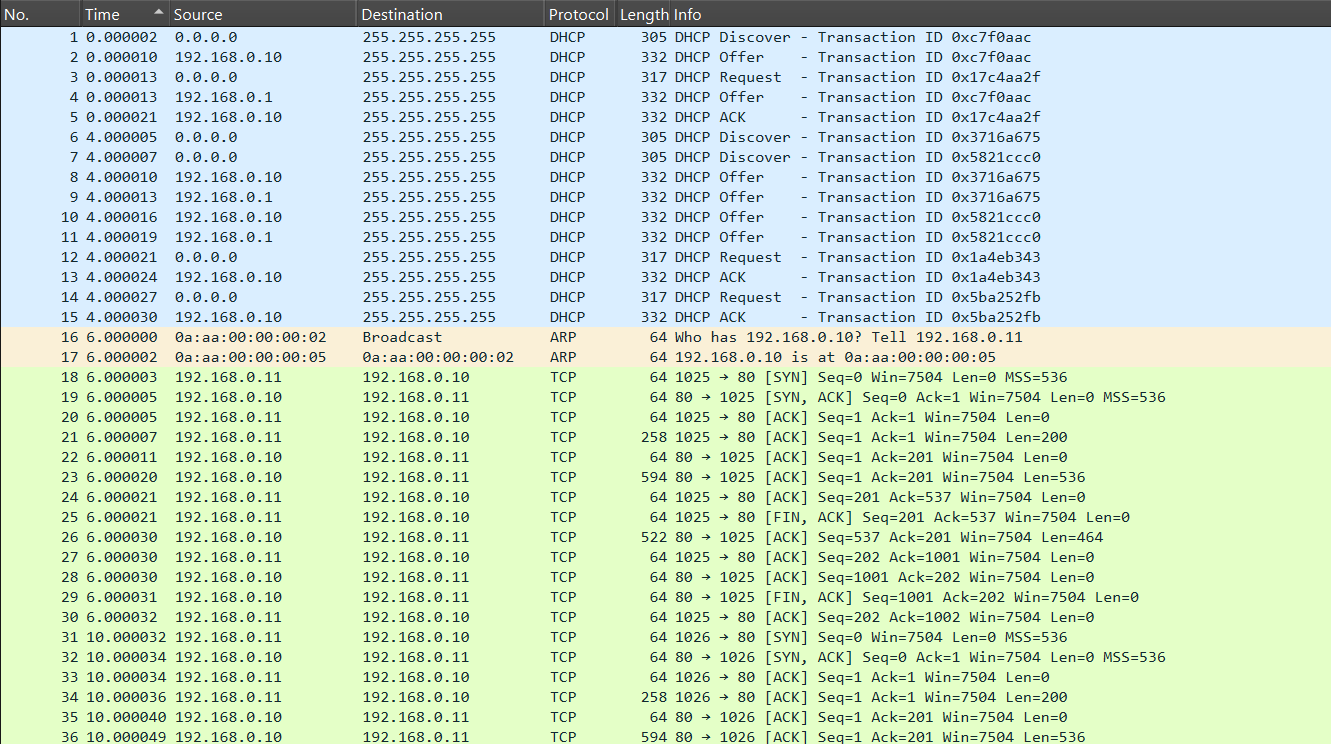
\includegraphics[width=135mm, scale=0.75]{imaxes/captura_ejer1_1.png}
    \caption{Tráfico DHCP entre host[0] y los servidores}
    \label{fig:captura_host0}
\end{figure}

Como podemos observar, el host[0] empieza haciendo un DHCP Discover para descubrir un servidor DHCP disponible. 
A continuación, el servidor local es el primero en responder la solicitud con un paquete DHCP Offer con una dirección IP disponible. El cliente (host[0]),
responde a su solicitud para confirmar la asignación ofrecida por el servidor local. El router también envía el paquete DHCP Offer, pero al enviarlo más tarde,
el cliente lo ignora. Finalmente, el servidor local contesta con un ACK (estos procesos se repiten para todos los cliente, host[1] y host[2]).

Posteriormente, el cliente host[0] intenta hacer la conexión con el servidor local, para lo cual manda primero un broadcast ARP, para asi saber 
cual es la MAC de la máquina, con la IP que establece en la cabecera ARP. Después, el servidor contesta al broadcast ARP que mandó el cliente identificandose
su mac, ya que la cabecera ARP incluye su IP.

Finalmente, la conexión sigue adelante con los mensajes de la Trasporte restableciendose cada 4 segundos, con


